\chapter{Algorithmes proposés}

\section{Introduction}

Dans le but d'identifier plus efficacement les réseaux moléculaires, nous présenterons dans ce chapitre les approches que nous proposons qui s'appuient sur les apprentissages ensemblistes Bagging et Boosting.
Le premier utilise l’approche \acrshort{Bagging} qui consiste à construire des échantillons aléatoirement de taille donnée, qui seront utilisés par des modèles de base pour construire des clusters, qui seront par la suite combinées par vote majoritaire.
Le deuxième utilise l’approche Boosting, qui par contre construit les échantillons en sélectionnant progressivement les observations mal regroupées par les weak-learner, en utilisant les clusters issues de \acrshort{GNPS} et \acrshort{MADByTE} comme oracle (vérité de regroupement).
Dans les deux méthodes, nous utilisons MCLA pour le vote majoritaire et pondéré.


\section{Méthode de type Bagging}

    Elle se déroule en plusieurs étapes suivantes qu'on peut retrouver sur la Figure \ref{fig:bio_bagging}:
    
   	 \subsection{Calcul des réseaux moléculaires}
  	 
		 Premièrement nous calculons les réseaux moléculaires issues des spectres MS et RMN en utilisant les solutions GNPS et MADByTE respectivement.
    
		 \subsection{Calcul des clusters contenus dans les réseaux moléculaires}
    
		 Pour détecter des groupes de molécules visibles sur un réseau moléculaire, les biologistes par nature repèrent les zones de forte densité de molécules y contenus.
 	 
		 Pour calculer ses clusters, nous utilisons l'algorithme \acrshort{DBSCAN} en définissant le voisinage d'une molécule comme étant l'ensemble des molécules connectées à lui dans le réseau moléculaire.
		 Vu que cette définition varie en fonction du type de réseau, nous avons le voisinage d'une molécule étant:
		 \begin{itemize}
 			  \item l'ensemble des molécules qui lui sont adjacents pour un réseau de GNPS
 			  \item l'ensemble les molécules qui partagent au moins un système de spin avec lui pour un réseau de MADByTE
   	 \end{itemize}
    
   	 \subsection{Transformation des spectres MS et RMN pour l'apprentissage multivues}

   	 Ici nous transformons les spectres MS et RMN en utilisant l'idée de l'outil MSPectraAI\footnote{Site officiel de l'outil MSPectraAI \href{ https://bio.tools/mspectraai }{ https://bio.tools/mspectraai } } qui est de définir des fenêtres de masse sur charge (de même taille) sur les spectres MS, puis d'agréger les intensités relatives y contenus pour obtenir un vecteur d'intensités indexé par les identifiants des fenêtres.

   	 Pour les spectres \acrshort{MS}, on définit un intervalle de valeur de masse sur charge de radicaux à considérer.
   	 Par la suite, nous segmentons le spectre d’entrée en fenêtres de même taille par rapport aux valeurs de masse sur charge.
   	 Chaque fenêtre obtenue va correspondre à une composante du vecteur final, cette composante qui contiendra la valeur agrégée (somme ou moyenne) des intensités relatives observées dans la fenêtre.

   	 Pour les spectres \acrshort{RMN}, on définit un intervalle de valeur de déplacement à considérer pour chaque type d'atomes considérés.
   	 Comme pour les spectres MS, on va segmenter le spectre RMN en fenêtres de même taille puis faire une agrégation des intensités.
   	 Ainsi si on a des spectres 2-RMN on aura en sortie une grille (vecteur ou matrice) d'intensité ou d'occurrence de croisement de déplacements. D’où le pseudo-algorithme:

    	\begin{algorithm}[H]
     		   \caption{Algorithme de prétraitement de spectres}
     		   \label{alg:molndbscan}
     		   \begin{algorithmic}[1]
     		   \REQUIRE spectre $s$, intervalles de déplacement $I$, fonction d'agrégation $arg$
            	\ENSURE vecteur $v$
		 
     		   \STATE $windows$ = split($s$, $I$);
            	\STATE $v$ = 0
            	\FORALL{i allant de 1 à $|windows|$}
                	$v[i]$ = arg($windows[i]$)
            	\ENDFOR
           	 
     		  \end{algorithmic}
     	  \end{algorithm}


   	 \subsection{Construction des clusters en utilisant la complémentarité et le consensus entre les spectres MS et RMN des molécules}

   	 Pour pouvoir tenir compte de la complémentarité et du consensus des spectres MS et RMN, nous utilisons comme algorithme de base \acrshort{MCLES} ou \acrshort{MVGL}, en introduisant lors du vote majoritaire (avec MCLA) les clusters détectés automatiquement sur les réseaux moléculaires venant de GNPS et MADByTE.
    	Pour chaque weak-learner fournissant les $K$ clusters voulus, on utilisera un échantillon construit par sélection aléatoire sans remise d'un pourcentage $p$ d'observations d'entrées.

   	 \subsection{Affectation des clusters aux réseaux moléculaires}

   	 Les clusters intégrant la complémentarité et le consensus des spectres MS et RMN, tout en tenant compte des clusters détectés par les biologistes, il nous faut les introduire dans les réseaux pour améliorer leur qualité.
   	 Pour le faire pour chaque molécule, nous ajoutons dans les méta-données de nœuds correspondants des réseaux obtenus (de GNPS et de MADByTE), son étiquette de cluster qui peut se caractériser visuellement par un coloriage ou une forme précise.

   	 \begin{figure}
   		 \begin{center}
       		 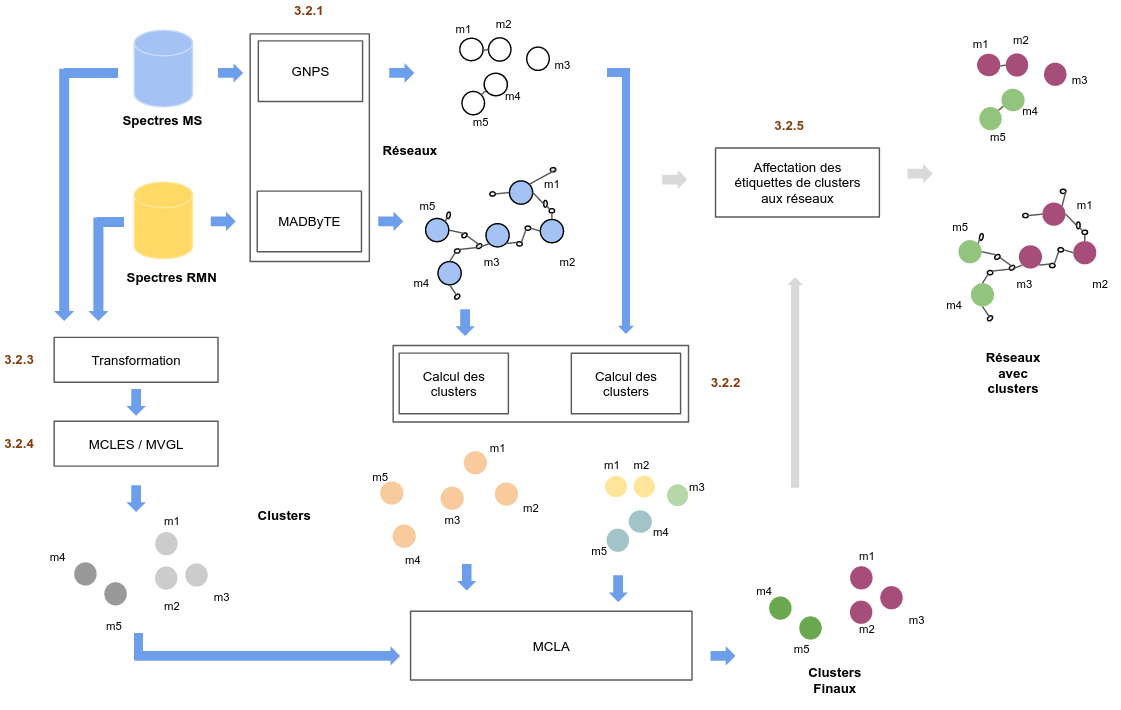
\includegraphics[width = \textwidth]{Images/bio_bagging.png}
   		 \end{center}
   		 \caption{Workflow de l'approche de type Bagging}
   		 \label{fig:bio_bagging}
   	 \end{figure}
  	 
	\section{Méthode de type Boosting}
  	 
   	 Cette méthode se déroule comme la précédente en modifiant l'étape de construction des clusters pour tenir compte de la complémentarité des spectres.
   	 Cette construction diffère de la méthode précédente par la méthode d'apprentissage par ensemble Boosting utilisée dont le workflow est représenté à la Figure \ref{fig:bio_bootsing}
  	 
   	 Nous adaptons l'algorithme Adaboost avec comme weak-learner  \acrshort{MCLES} ou  \acrshort{MVGL}, pour permettre de construire itérativement des clusters de meilleurs qualités par échantillonnage d'observations.
   	 Nous considérons qu'une observation est \textbf{bien classée} (ou encore bien regroupée) quand toutes les molécules du même cluster que lui par rapport au weak-learner, le sont aussi par rapport aux réseaux moléculaires issues de GNPS et MADByTE.
   	 Les clusters extraites des réseaux de GNPS et de MADByTE deviennent ainsi des oracles permettant de s'assurer que les modèles de base intègrent progressivement leurs constructions.
  	 
   	 \begin{figure}
   		 \begin{center}
       		 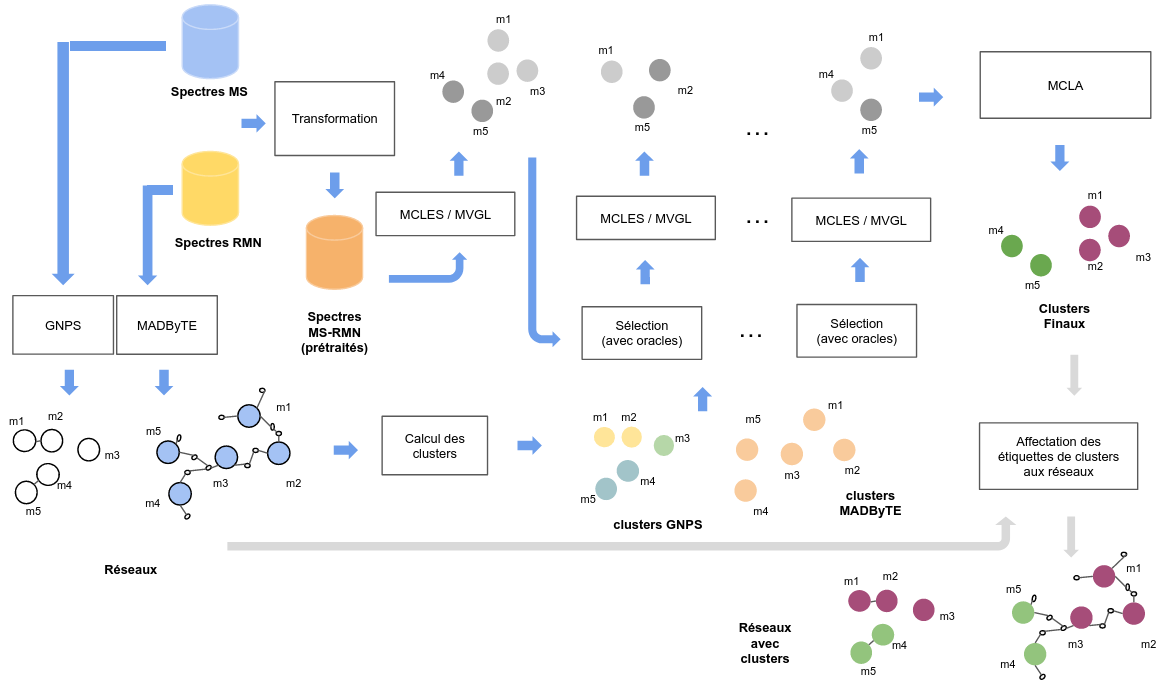
\includegraphics[width = \textwidth]{Images/bio_bootsing.png}
   		 \end{center}
   		 \caption{Workflow de l'approche de type Boosting}
   		 \label{fig:bio_bootsing}
   	 \end{figure}
  	 
  	 
   	 \section{Conclusion}
  	 
   	 En définitive, il était question pour nous de présenter les approches proposées pour accélérer l'identification des molécules en laboratoire, en regroupant leurs spectres MS et RMN en tenant compte de leur complémentarité et de leur potentiel consensus, ce qui permet par ricochet d'identifier les réseaux moléculaires les contenant.
    	Dans la suite nous réaliserons les expérimentations sur la méthode de type Bagging en s'appuyant sur l'étape de construction des clusters.
   	 